\chapter{Implementation and analysis of a POD-DEIM reduced model for the optimal control of Burgers' equation}
\label{chap4}
In \cite{KV99}, the authors used a POD-reduced model for the optimal control of Burgers' equation. In this Section, we extend this approach by applying model order reduction using POD-DEIM as described in Section \ref{MOR_chap} to an optimal control problem as described in Section \ref{Opt_chap} and compare the POD-DEIM reduced model to the POD model in terms of computational cost and accuracy. The reduced optimal control problem is in the implicitly-constrained form,
\begin{equation}
\label{allgControl_small}
\begin{split}
\min_{u} \ &\tilde{\mathcal{J}}(\tilde{y}(u),u) ,\\
\text{with } \ &\tilde{c}(\tilde{y},u) = 0,
\end{split}
\end{equation}
where we use a tilde to indicate that the considered quantity is of lower dimension. In \eqref{allgControl_small}, the constraining nonlinear PDE $\tilde{c}(\tilde{y},u) = 0$ is solved for the reduced state variable $\tilde y(u)$. Since the evaluation of the cost function $\tilde{\mathcal{J}}$ requires the computation of $\tilde{y}$ first, this approach also leads to a faster evaluation of the cost function due to the lower dimension of the state variable. We will refer to the solution of \eqref{allgControl_small} as the optimal control of the reduced system. It is important to note, that even though this optimal control is derived from the reduced system, we denote it without tilde in order to stress that the control is still of the large dimension of the full-order model. This is a natural approach at this point because $u$ can be seen as an input variable because the state $\tilde{y}(u)$ directly depends on the control. A dimension reduction of the control $u$ is not considered at this point. Similarly to the previous section, we denote by $\hat{\tilde{\mathcal J}}(u) := \tilde{\mathcal{J}}(\tilde{y}(u),u)$ the cost function as a function of the control only.
\newpage
\section{A POD-DEIM reduced model for optimal control of Burgers' equation}
\label{redOptimalControl}
In Section \ref{fullOrderControl}, we introduced the optimal control problem \eqref{minJ}-\eqref{Burgers2}. We will now derive a POD-DEIM reduced model of the corresponding discrete optimization problem \eqref{minJ_discr}-\eqref{Burgers2_discr}. Therefore, we first consider the discretized objective function \eqref{minJ_discr} and recall that the reduced state variable has been derived in the following way,
\begin{align*}
\mathbf{y}(t) \approx \Phi_\ell \mathbf{\tilde y}(t),
\end{align*}
where the columns of the matrix $\Phi_\ell$ are the POD basis. When we plug in this approximation into \eqref{minJ_discr}, we obtain the reduced objective function,
\begin{align}
\label{redOpt}
\min_{\mathbf{u}_0,...,\mathbf{u}_{N_t}} \tilde{J}(\mathbf{\tilde y}_0,...,\mathbf{\tilde y}_{N_t},\mathbf{u}_0,...,\mathbf{u}_{N_t}) = \min_{\mathbf{u}_1,...,\mathbf{u}_{N_t}} \sum_{i=0}^{N_t} \delta \! t \left( \frac{1}{2} \mathbf{\tilde y}_i^T \mathbf{\tilde y}_i - \mathbf{\tilde z}^T\mathbf{\tilde y}_i + \frac{\omega}{2}\mathbf{u}_i^T M \mathbf{u}_i \right),
\end{align}
where the mass matrix in the first term vanishes due to the M-orthogonality of $\Phi_\ell$ and the reduced desired state $\mathbf{\tilde z}$ is given by,
\begin{align}
\label{zred}
\mathbf{\tilde z} &:= \Phi_\ell^T \mathbf{z} \in \mathbb{R}^\ell.
\end{align}
Note that \eqref{zred} can be pre-computed once the POD basis is obtained because the desired state of the full-order model is a given function, see \eqref{fullz}. We further note problem \eqref{redOpt} is still formulated in terms of the full-dimensional control $\mathbf{u}_i$ at the time instances $t_i$. In Section \ref{smallu_sec}, we will show one way in which a lower-dimensional control can lead to a reduced model that is completely independent of the full-order dimension $N$.

In order to obtain a POD-DEIM reduced model for the constraining Burgers' equation, we refer to Section \ref{fullOrderControl} and apply the POD-DEIM projection to \eqref{Burgers2_discr}. The fully discretized reduced constraint is, thus, given by
\begin{align}
\label{redBurgers}
\tilde{c}_i(\mathbf{\tilde y}_i,\mathbf{\tilde y}_{i+1},\mathbf{u}_{i+1}) \equiv \frac{1}{\delta \! t} \mathbf{\tilde y}_{i+1} - \frac{1}{\delta \! t}\mathbf{\tilde y}_i + \frac{1}{2} \tilde{B}(\tilde{F}\mathbf{\tilde y}_{i+1})^2 + \nu \tilde{C}\mathbf{\tilde y}_{i+1} - \mathbf{\tilde f} - \tilde{M} \mathbf{u}_{i+1} = 0,
\end{align}
where $i=0,...,N_t-1$ and a dimension reduction for the right-hand side as well as the projected mass matrix has been obtained,
\begin{align}
\label{fred}
\mathbf{\tilde f} &:= \Phi_\ell^T \mathbf{f} \in \mathbb{R}^\ell,\\
\label{M1red}
\tilde{M} &:= \Phi_\ell^T M \in \mathbb{R}^{\ell \times N}.
\end{align}
Note that $\tilde{M}$ still depends on $N$ and the matrices $\tilde{B}, \tilde{C}, \tilde{F}$ have been defined in \eqref{Bred}, \eqref{Cred}, \eqref{Fred}, respectively.

Furthermore, we note that the nonlinear term in \eqref{redBurgers} has to be considered as a function of the reduced variable $\mathbf{\tilde y}$ and has the slightly more complicated form,
\begin{align}
 \label{redNonlin}
 \tilde{\mathcal{N}}(\mathbf{\tilde{y}}_{i+1}) := \frac{1}{2} \tilde{B} (\tilde{F} \mathbf{\tilde{y}}_{i+1})^2.
\end{align}

The Lagrangian function of the reduced model can be obtained directly from \eqref{redOpt} and \eqref{redBurgers} and is given by,
\begin{align}
\label{redLag}
&\mathcal{\tilde L}(\mathbf{\tilde y}_0,...,\mathbf{\tilde y}_{N_t}, \mathbf{u}_0,...,\mathbf{u}_{N_t},\boldsymbol{\tilde \lambda}_1,...,\boldsymbol{\tilde \lambda}_{N_t}) \nonumber \\
&\ = \sum_{i=0}^{N_t} \delta \! t \left( \frac{1}{2} \mathbf{\tilde y}_i^T \mathbf{\tilde y}_i - \mathbf{\tilde z}^T\mathbf{\tilde y}_i + \frac{\omega}{2} \mathbf{u}_i^T M \mathbf{u}_i \right) \nonumber \\
&\quad +  \sum_{i=0}^{N_t-1} \boldsymbol{\tilde \lambda}_{i+1}^T \left( \frac{1}{\delta \! t} \mathbf{\tilde y}_{i+1} - \frac{1}{\delta \! t} \mathbf{\tilde y}_i + \frac{1}{2} \tilde{B} (\tilde{F} \mathbf{\tilde y}_{i+1})^2 + \nu \tilde{C} \mathbf{\tilde y}_{i+1} - \mathbf{\tilde f} - \tilde{M} \mathbf{u}_{i+1}  \right)
\end{align}
In \eqref{redLag}, we see that the adjoint variable $\boldsymbol{\tilde \lambda}_i \in \mathbb{R}^\ell$ is of the same dimension $\ell$ as the reduced state variable. This gives a good motivation for a faster solution of the adjoint equations \eqref{adjoint1} when applied to the POD-DEIM reduced model.
\section{A Newton-type method for the POD-DEIM reduced model}
\label{Newton_red_chapter}
In Section \ref{NumTests_Hess}, we have already seen that the application of the adjoints for derivative computation according to Algorithm \eqref{alg:Adj1} and \eqref{alg:Adj2} is straightforward but the derivation of partial derivatives of the nonlinear term is still involved when applied to a concrete problem. In Algorithm \ref{alg:Adj1_redBurgers}, we present the computation of the gradient of the reduced objective function which follows from the application of Algorithm \ref{alg:Adj1} to the reduced model \eqref{redOpt}-\eqref{redBurgers}.
\begin{algorithm}[H]
\caption{Algorithm \ref{alg:Adj1} applied to the reduced Burgers' model}
\label{alg:Adj1_redBurgers}
\begin{algorithmic}[1]
\STATE From the initial condition $\mathbf{\tilde y}_0$ and the current control $\mathbf{u}_0,...,\mathbf{u}_{N_t}$, solve the reduced Burgers' equation for $\mathbf{\tilde y}_1,...,\mathbf{\tilde y}_{N_t}$ according to \ref{redBurgers}
\STATE The adjoint equation \eqref{adjoint1} reads:
\begin{subequations}
\begin{align}
\label{AdjRedOrder_term}
\left(\frac{1}{\delta \! t}I_\ell + \tilde{\mathcal{N}}'(\mathbf{\tilde{y}}_{N_t})  +  \nu \tilde{C}\right)^T \boldsymbol{\tilde{\lambda}}_{N_t} &= -\delta \! t(\mathbf{\tilde{y}}_{N_t} - \mathbf{\tilde z} )\\
\label{AdjRedOrder}
\left(\frac{1}{\delta \! t}I_\ell + \tilde{\mathcal{N}}'(\mathbf{\tilde{y}}_{i})  + \nu \tilde{C}\right)^T \boldsymbol{\tilde{\lambda}}_i &= - (-\frac{1}{\delta \! t} I_\ell)^T \boldsymbol{\tilde{\lambda}}_{i+1} -\delta \! t( \mathbf{\tilde{y}}_{i} - \mathbf{\tilde z} ), \quad i = N_t-1,...,1
\end{align}
\end{subequations}
\STATE The gradient is computed according to formula \eqref{grad}:
\begin{align}
\label{gradRedOrder}
\nabla \hat{\tilde{\mathcal J}}(\mathbf{u}_0,...,\mathbf{u}_{N_t}) = \begin{pmatrix} \delta \! t \omega M \mathbf{u}_0 \\ \delta \! t \omega M \mathbf{u}_1 - \tilde{M}^T \boldsymbol{\tilde{\lambda}}_1 \\ \vdots \\ \delta \! t \omega M \mathbf{u}_{N_t} - \tilde{M}^T \boldsymbol{\tilde{\lambda}}_{N_t} \end{pmatrix}
\end{align}
\end{algorithmic}
\end{algorithm}
Because of the small dimension of the adjoint variable $\boldsymbol{\tilde{\lambda}}_i$, we note that the solution of the linear systems \eqref{AdjRedOrder_term}-\eqref{AdjRedOrder} can be obtained much faster than in the full-order case. In \eqref{AdjRedOrder_term} and \eqref{AdjRedOrder} and the remainder of the paper, $I_\ell$ denotes the identity matrix of dimensions $\ell \times \ell$. It is important to stress that the Jacobian of the nonlinearity \eqref{redNonlin} has to be computed in terms of the reduced variable $\mathbf{\tilde y}$ and is, hence, of dimension $\ell \times \ell$ as the the following computation shows:
\begin{align}
\label{Jac_non_red}
\tilde{\mathcal{N}}'(\mathbf{\tilde{y}}) = \frac{d}{d \mathbf{\tilde{y}}} \left( \frac{1}{2} \tilde{B} (\tilde{F}\mathbf{\tilde{y}})^2 \right) = \begin{pmatrix} \tilde{B}_{1,1} & \hdots & \tilde{B}_{1,m}\\ \vdots & & \vdots \\ \tilde{B}_{\ell,1} & \hdots & \tilde{B}_{\ell,m}  \end{pmatrix} \cdot \begin{pmatrix} \mathbf{\langle \tilde{y}} , \tilde{F}_1\rangle \tilde{F}_{1,1} & \hdots & \langle \mathbf{\tilde{y}} , \tilde{F}_1 \rangle \tilde{F}_{1,\ell} \\ \vdots & & \vdots \\ \langle \mathbf{\tilde{y}} , \tilde{F}_m \rangle \tilde{F}_{m,1} & \hdots & \langle \mathbf{\tilde{y}}. \tilde{F}_m \rangle \tilde{F}_{m,\ell}  \end{pmatrix}.
\end{align}
In \eqref{Jac_non_red}, we denoted by $\tilde{F}_i$ the $i$-th row of the matrix $\tilde{F}$ and $\tilde{B}_{i,j}, \tilde{F}_{i,j}$ denotes the entry of the respective matrix at position $i,j$. Here, $\langle \cdot , \cdot \rangle$ stands for the standard scalar product in $\mathbb{R}^\ell$. Note that because of the full dimension of $\mathbf{u}_i$, the gradient in \eqref{gradRedOrder} is still of dimension $N \cdot N_t \times 1$. Algorithm \ref{alg:Adj1_redBurgers} has also been used for the gradient computation that is required for the first-order optimization methods SPG and BFGS.

We next present the efficient computation of the Hessian-times-vector product $\nabla^2 \hat{\tilde{\mathcal J}} \cdot \mathbf{\underline{v}}$ using adjoints. Since the Hessian with respect to $u$ is of dimension $N \cdot N_t \times N \cdot N_t$, the corresponding vector used in Algorithm \ref{alg:Adj2_redBurgers} is of the following form, $\mathbf{\underline{v}} := (\mathbf{v}_0, ..., \mathbf{v}_{N_t})^T \in \mathbb{R}^{(N \cdot N_t) \times 1}$.
\begin{algorithm}[H]
\caption{Algorithm \ref{alg:Adj2} applied to the reduced Burgers' model}
\label{alg:Adj2_redBurgers}
\begin{algorithmic}[1]
\STATE We assume that we have already computed $\mathbf{\tilde{y}}_0,...,\mathbf{\tilde{y}}_{N_t}, \mathbf{u}_0,...,\mathbf{u}_{N_t},\boldsymbol{\tilde{\lambda}}_1,...,\boldsymbol{\tilde{\lambda}}_{N_t}$ in \mbox{Algorithm \ref{alg:Adj1_redBurgers}}
\STATE Equation \eqref{eqnw} reads:
\begin{subequations}
\begin{align}
\label{wRedOrder_init}
\mathbf{\tilde{w}}_0 &= 0 \\
\label{wRedOrder}
\left( \frac{1}{\delta \!t} I_\ell + \tilde{\mathcal{N}}'(\mathbf{\tilde{y}}_{i+1})  + \nu \tilde{C}\right) \mathbf{\tilde{w}}_{i+1} &=  - (-\frac{1}{\delta \! t}I_\ell)\mathbf{\tilde{w}}_i - \tilde{M}\mathbf{v}_{i+1} , \quad i = 0,...,N_t-1
\end{align}
\end{subequations}
\STATE Equation \eqref{eqnp} reads:
\begin{subequations}
\begin{align}
\label{pRedOrder_term}
\left( \frac{1}{\delta \!t} I_\ell + \tilde{\mathcal{N}}'(\mathbf{\tilde{y}}_{N_t})  + \nu \tilde{C} \right)^T \mathbf{\tilde{p}}_{N_t} &= \delta \! t I_\ell \mathbf{\tilde{w}}_{N_t} + \left( \tilde{\boldsymbol \lambda}_{N_t}^T \tilde{\mathcal{N}}(\mathbf{\tilde{y}}_{N_t}) \right)'' \mathbf{\tilde{w}}_{N_t} \\
\label{pRedOrder}
\left( \frac{1}{\delta \!t} I_\ell + \tilde{\mathcal{N}}'(\mathbf{\tilde{y}}_{i})  + \nu \tilde{C} \right)^T \mathbf{\tilde{p}}_{i} &=  -(-\frac{1}{\delta \! t}I_\ell)^T\mathbf{\tilde{p}}_{i+1} + \delta \! t I_\ell \mathbf{\tilde{w}}_i + \left( \tilde{\boldsymbol \lambda}_{i}^T \tilde{\mathcal{N}}(\mathbf{\tilde{y}}_{i}) \right)'' \mathbf{\tilde{w}}_{i}, \quad i = N_t-1,...,1
\end{align}
\end{subequations}
\STATE The Hessian times a vector $\mathbf{\underline{v}}$ is computed according to formula \eqref{hesseqn}:
\begin{align}
\label{HessRedOrder}
\nabla^2 \hat{\tilde{\mathcal{J}}}(\mathbf{u}_0,...,\mathbf{u}_{N_t}) \mathbf{\underline{v}} = \begin{pmatrix} \delta \! t \omega M \mathbf{v}_0 \\ -\tilde{M}^T \mathbf{\tilde{p}}_1 + \delta \! t \omega M \mathbf{v}_1\\ \vdots \\ -\tilde{M}^T \mathbf{\tilde{p}}_{N_t} + \delta \! t \omega M \mathbf{v}_{N_t} \end{pmatrix}
\end{align}
\end{algorithmic}
\end{algorithm}
\newpage
Note that the second partial derivative of the nonlinear term $\tilde{\boldsymbol \lambda}^T \tilde{\mathcal{N}}(\mathbf{\tilde{y}})$ with respect to the reduced variable $\mathbf{\tilde{y}}$ in step $3$ of the above algorithm is given by:
\begin{align*}
\frac{d^2}{d\mathbf{\tilde y}^2} \left( \tilde{\boldsymbol \lambda}^T \tilde{\mathcal{N}}(\mathbf{\tilde{y}}) \right) \mathbf{\tilde{w}} &=  \frac{d^2}{d\mathbf{\tilde y}^2} \left( \boldsymbol{\tilde{\lambda}}^T (\frac{1}{2} \tilde{B} (\tilde{F} \mathbf{\tilde{y}})^2) \right) \mathbf{\tilde{w}}
=\frac{d^2}{d\mathbf{\tilde y}^2} \left( \sum_{k=1}^\ell \lambda_k \frac{1}{2} \sum_{j=1}^m \tilde{B}_{k,j} \left( \sum_{i=1}^\ell \tilde{F}_{j,i}\tilde{y}_i \right)^2 \right) \mathbf{\tilde{w}} \\
&= \frac{d}{d\mathbf{\tilde y}} \begin{pmatrix} \sum_{k=1}^\ell \lambda_k \sum_{j=1}^m \tilde{B}_{k,j} \sum_{i=1}^\ell \tilde{F}_{j,i}\tilde{y}_i \cdot \tilde{F}_{j,1}\\ \vdots \\ \sum_{k=1}^\ell \lambda_k \sum_{j=1}^m \tilde{B}_{k,j} \sum_{i=1}^\ell \tilde{F}_{j,i}\tilde{y}_i \cdot \tilde{F}_{j,\ell} \end{pmatrix}\mathbf{\tilde{w}} \\
&= \underbrace{\begin{pmatrix} \sum_{k=1}^\ell \lambda_k \sum_{j=1}^m \tilde{B}_{k,j} \tilde{F}_{j,1} \tilde{F}_{j,1} & \hdots & \sum_{k=1}^\ell \lambda_k \sum_{j=1}^m \tilde{B}_{k,j} \tilde{F}_{j,\ell} \tilde{F}_{j,1}\\ \vdots & & \vdots \\ \sum_{k=1}^\ell \lambda_k \sum_{j=1}^m \tilde{B}_{k,j} \tilde{F}_{j,1} \tilde{F}_{j,\ell} & \hdots & \sum_{k=1}^\ell \lambda_k \sum_{j=1}^m \tilde{B}_{k,j} \tilde{F}_{j,\ell} \tilde{F}_{j,\ell} \end{pmatrix}}_{\in \mathbb{R}^{\ell \times \ell}} \mathbf{\tilde{w}}
\end{align*}
Due to the dimensions of the reduced variables, it is natural that the above matrix-times-vector product only depends on the dimension $\ell$. The matrix is not constant in time because the adjoint variable depends on time and can, thus, not be pre-computed. An efficient implementation is therefore necessary in order to obtain a computational speedup if $\ell \ll N$.

Algorithm \ref{alg:Opt+MOR1} gives an overview of the optimization algorithm that has been developed for the optimal control of the POD-DEIM reduced model of Burgers' equation. Algorithm \ref{alg:Opt+MOR1} is an iterative procedure to update the reduced model aiming to improve the approximation to the full-order model. The procedure is as follows: In order to obtain snapshots, it is necessary to solve the full-order model corresponding to an initial control once. From snapshots of the full-order solution, we can derive the reduced model and solve the \textit{reduced} optimization problem for an optimal control. The reduced model can be improved in an iterative process by obtaining new snapshots of the state corresponding to the current optimal control. Then, a new POD-DEIM model is derived from the new snapshots and the same optimization algorithm is applied to the improved reduced model. This can be repeated until a certain stopping criterion is satisfied. In Algorithm \ref{alg:Opt+MOR1}, we improve the reduced model as long as the obtained optimal state is close enough to the desired state $z$ measured in the $L_2$-norm. Another approach for stopping could be that the reduced objective function reaches the value of the objective function of the full-order model evaluated at the optimal state. This, however, is only possible if the full-order optimal control has already been solved which we want to avoid in our implementation.
\newpage
\begin{algorithm}[H]
\caption{Optimal control: Iterative improvement of the reduced model}
\label{alg:Opt+MOR1}
\begin{algorithmic}[1]
\STATE Set initial control $u^{(0)} = 0$, and $K = 0$, $\varepsilon_z \in \mathbb{R}_+$, \texttt{max\_iter} $\in \mathbb{N}$
\STATE Solve the full-order Burgers' equation $c(y^{(0)},u^{(0)})$ for the uncontrolled state $y^{(0)}$ via \eqref{Burgers2_discr}
\STATE Choose POD dimension $\ell$ and DEIM-dimension $m$
\WHILE{$\|y^{(K)}-z\|_{L^2([0,L] \times [0,T])} > \varepsilon_z$ \AND $K < $\texttt{max\_iter}}
\STATE Obtain the POD-DEIM reduced model from snapshots of $y^{(K)}$, i.e. compute $\Phi_\ell$ via \eqref{Phidef} and $\mathcal{P}$ via Algorithm \ref{alg:DEIM}
\STATE Calculate reduced optimal control, $u^{(K+1)} = \argmin_u \tilde{\mathcal J}(\tilde{y}(u),u)$ by solving the reduced optimization problem \eqref{redOpt} with implicit constraint \eqref{redBurgers}. Choose one of the optimization algorithms \ref{alg:Opt}, \ref{alg:BFGS} or \ref{alg:SPG}.
\STATE Solve the reduced Burgers' equation $\tilde{c}(\tilde{y}^{(K+1)},u^{(K+1)}) = 0$ for $\tilde{y}^{(K+1)}$ via \eqref{redBurgers}
\STATE Expand $y^{(K+1)} = \Phi_\ell \tilde{y}^{(K+1)}$
\STATE $K = K + 1$
\ENDWHILE
\end{algorithmic}
\end{algorithm}
In Figure \ref{optred}, we show numerical results for the optimal control of Burgers' equation using a POD-DEIM reduced model of different dimensions $\ell$ and $m$ and using the Newton-type method of Algorithm \ref{alg:Opt} for solving the optimization problem. We see that due to the low-dimensional state variable, the desired state is not reached with the same accuracy as in the full-order case. This leads to a larger optimal value of the objective function \eqref{redOpt} as the results in Section \ref{numTests} will show.
\begin{figure}[H]
\centering
\subfloat[$\ell = m = 7$]{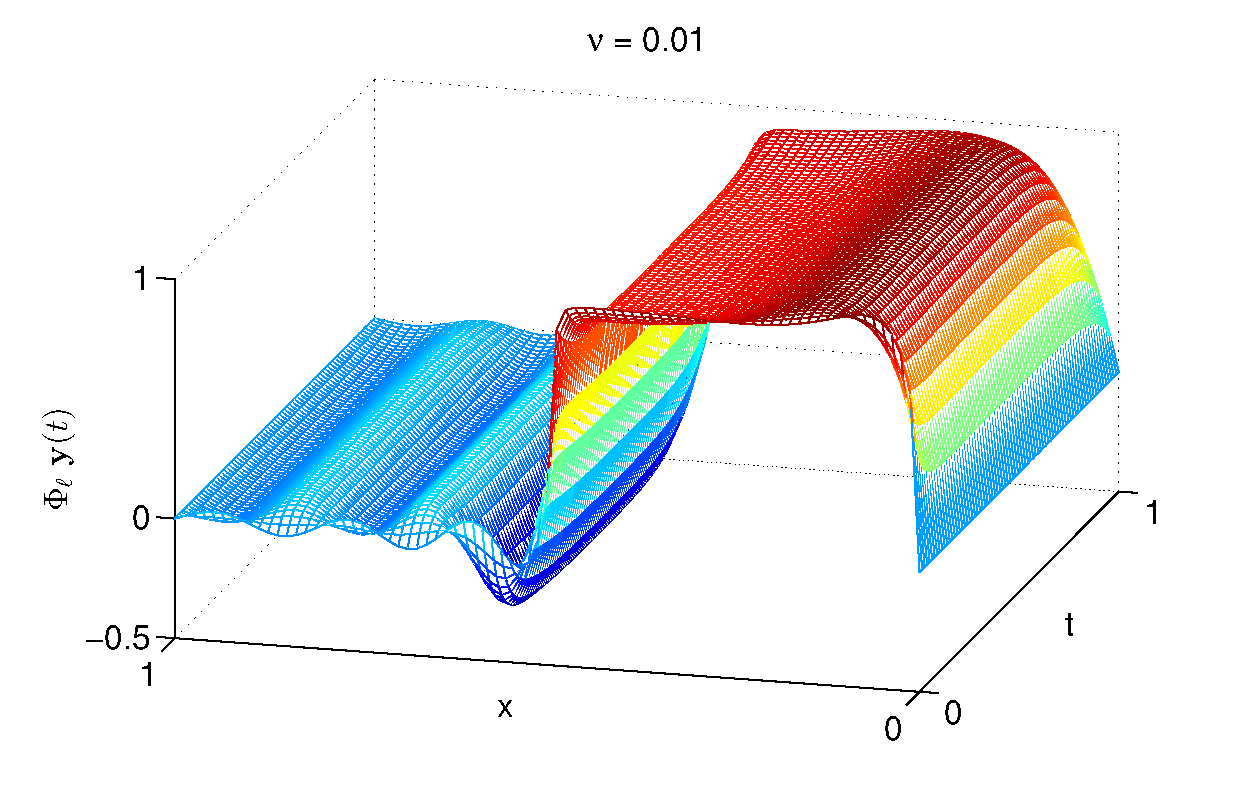
\includegraphics[width=0.49\textwidth]{plots/redOptCon_y7}}\hfill
\subfloat[$\ell = m = 15$]{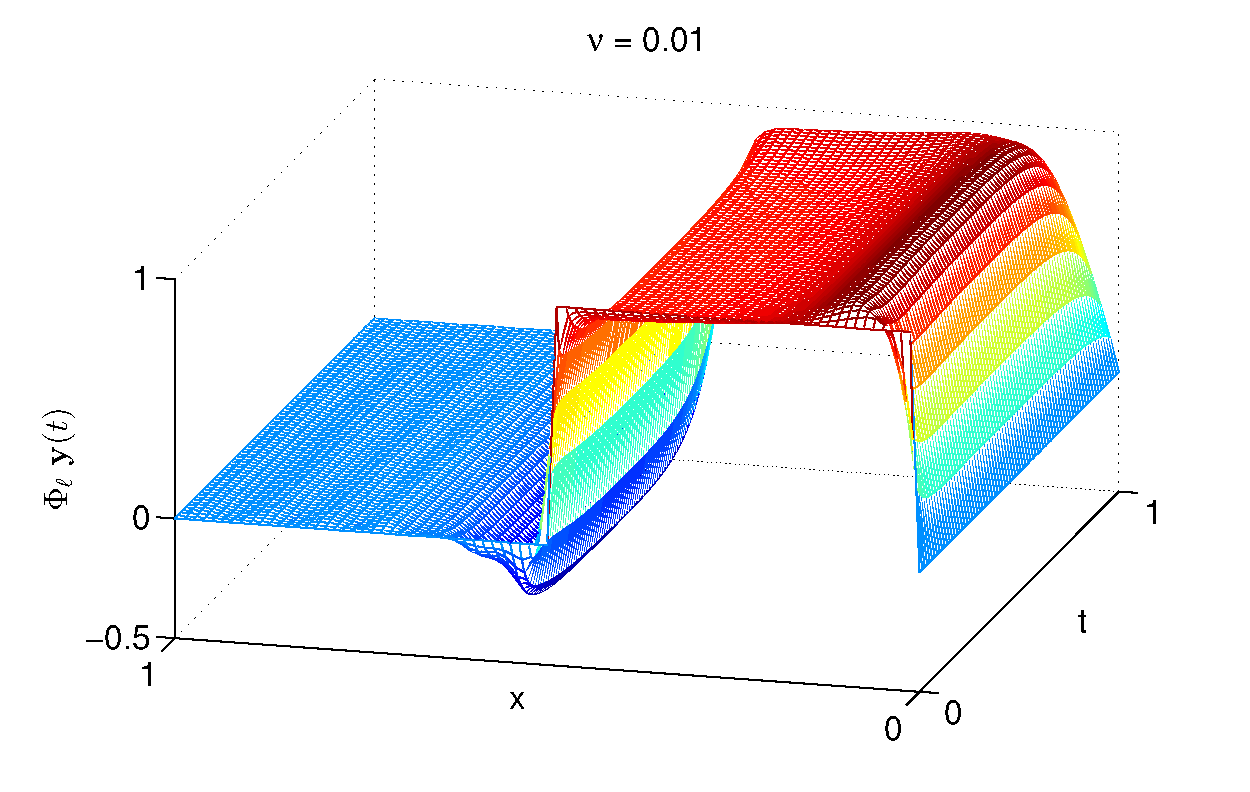
\includegraphics[width=0.49\textwidth]{plots/redOptCon_y15}}\\
\subfloat[$\ell = m = 7$ ]{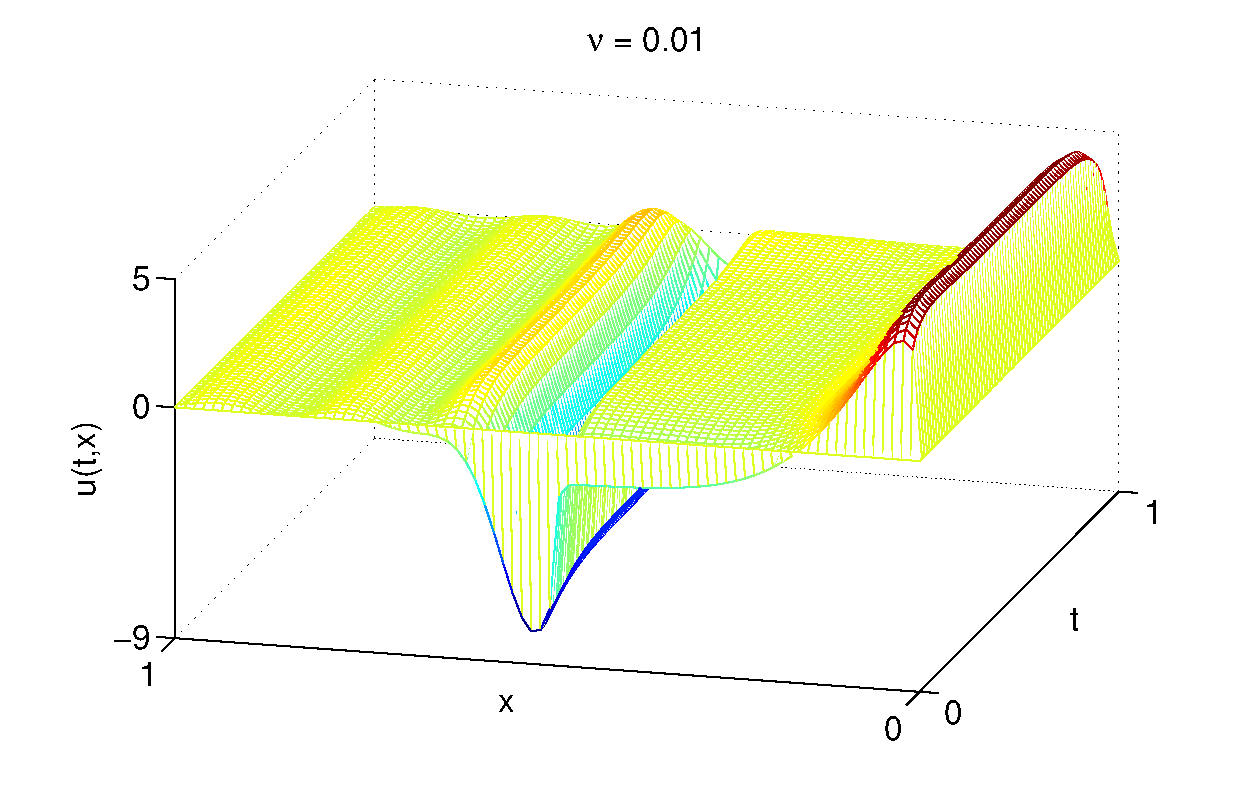
\includegraphics[width=0.49\textwidth]{plots/redOptCon_u7}}\hfill
\subfloat[$\ell = m = 15$]{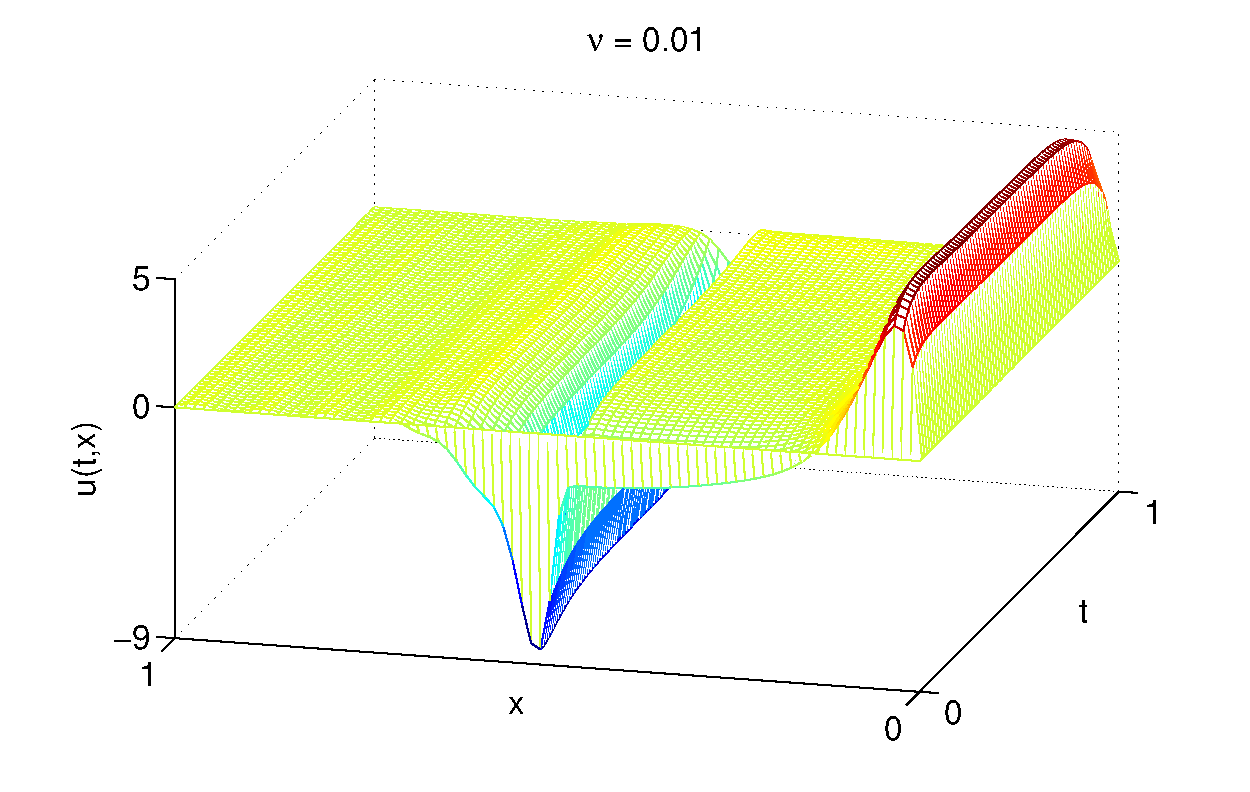
\includegraphics[width=0.49\textwidth]{plots/redOptCon_u15}}\\
\caption{Optimal control of the POD-DEIM reduced Burgers' model using different dimensions.}\label{optred}
\end{figure}
%\begin{algorithm}[H]
%\caption{Optimal control: Improving the reduced model using the full-order system}
%\label{alg:Opt+MOR}
%\begin{algorithmic}[1]
%\STATE Set initial control $\mathbf{\underline{u}}^{(0)} = 0$, and $k = 0$, $tol \in \mathbb{R}_+$, \texttt{MAX\_FULL} $\in %\mathbb{N}$
%\STATE Solve the full-order Burgers' equation \eqref{Burgers2_discr} for $\mathbf{\underline{y}}^{(0)}$ (uncontrolled %state)
%\WHILE{$k <$ \texttt{MAX\_FULL}}
%\STATE Set $\mathbf{\underline{u}}_{\text{old}} = \mathbf{\underline{u}}^{(k)}$
%\STATE Obtain the POD-DEIM reduced model from snapshots of $\mathbf{\underline{y}}^{(k)}$ and %$\mathbf{\underline{u}}^{(k)}$, i.e compute $\Phi_\ell$ via \eqref{Phidef}, $\Psi_\ell$ via \eqref{Psidef} and %$\mathcal{P}$ via Algorithm \ref{alg:DEIM}
%\STATE Calculate reduced control $\mathbf{\underline{\tilde u}}^{(k+1)}$ by solving the reduced optimization problem %\eqref{redOpt} subject to \eqref{redBurgers} via Algorithm \ref{alg:Opt}
%\STATE Set $\mathbf{\underline{u}}_{\text{new}} = \text{blkdiag}(\Psi_\ell)\mathbf{\underline{\tilde u}}^{(k+1)}$
%\IF{$\|\mathbf{\underline{u}}_{\text{old}} - \mathbf{\underline{u}}_{\text{new}}\| < tol$}
%\RETURN
%\ELSE
%\STATE Calculate full-order control $\mathbf{\underline{u}}^{(k+1)}$ by solving the optimization problem \eqref{minJ_discr} %subject to \eqref{Burgers2_discr} via Algorithm \ref{alg:Opt}
%\ENDIF
%\STATE $k = k + 1$
%\ENDWHILE
%\end{algorithmic}
%\end{algorithm}

%\begin{figure}[H]
%\centering
%\subfloat[$k=1$ (uncontrolled)]{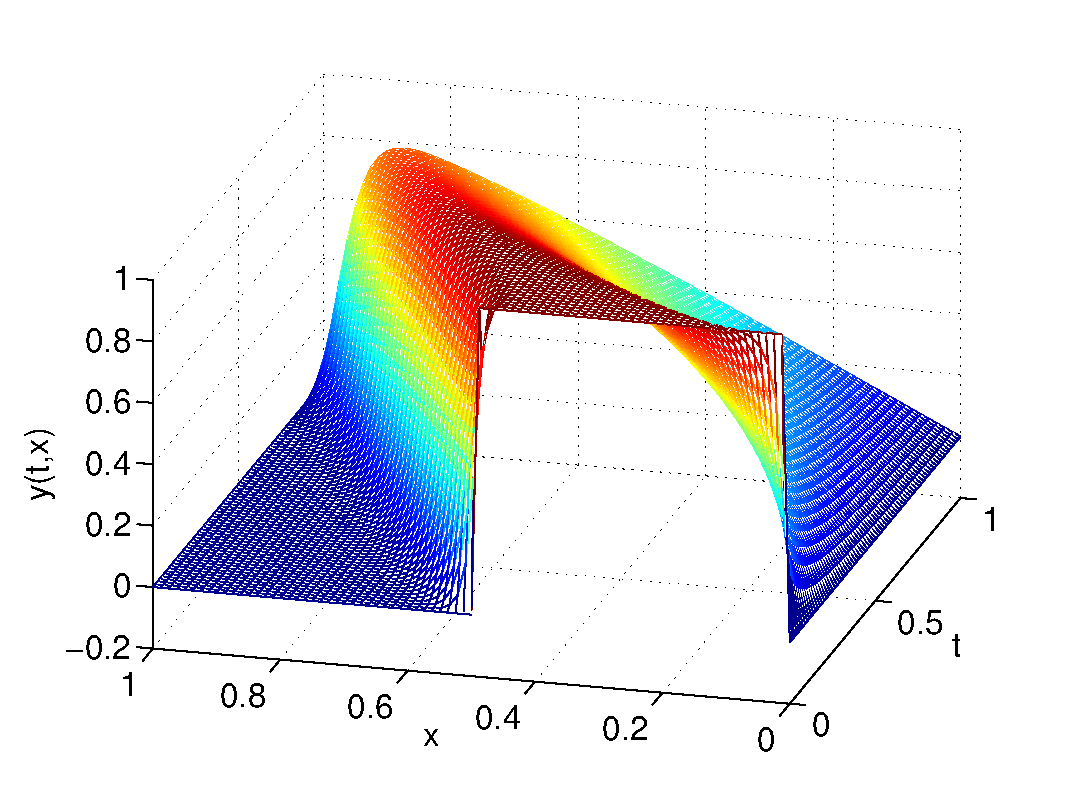
\includegraphics[width=0.49\textwidth]{plots/controlRedk1}}\hfill
%\subfloat[$k=2$]{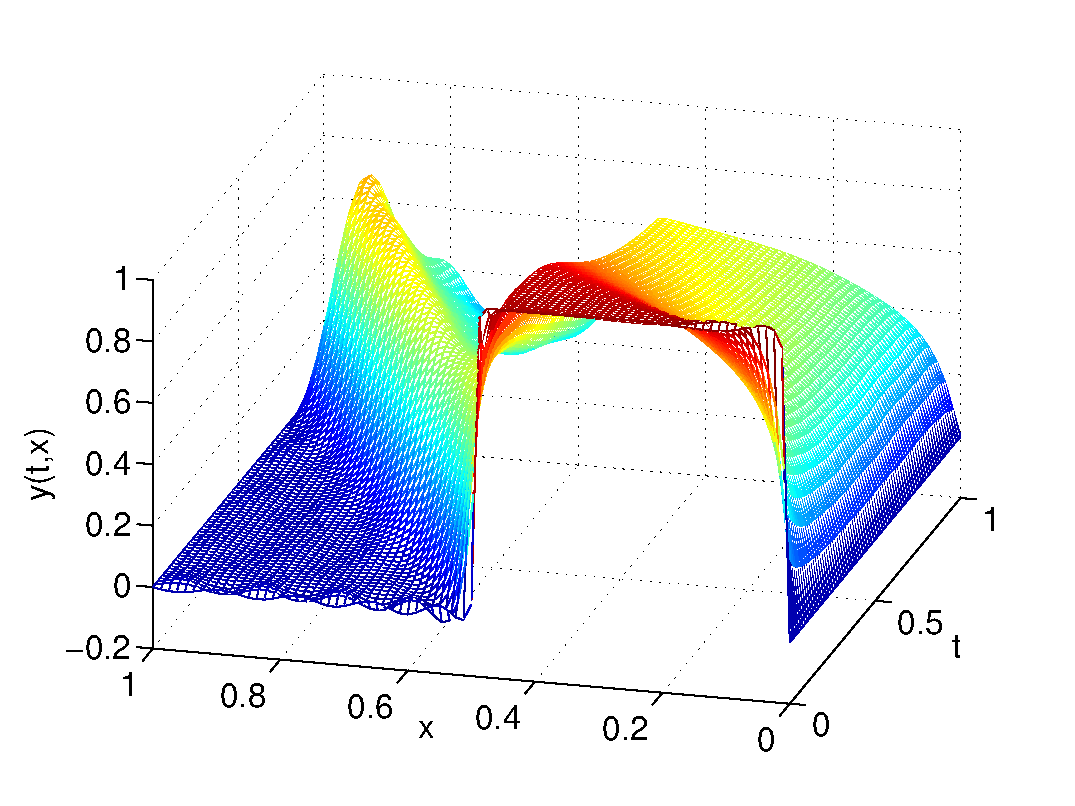
\includegraphics[width=0.49\textwidth]{plots/controlRedk2}}\\
%\subfloat[$k=5$ ]{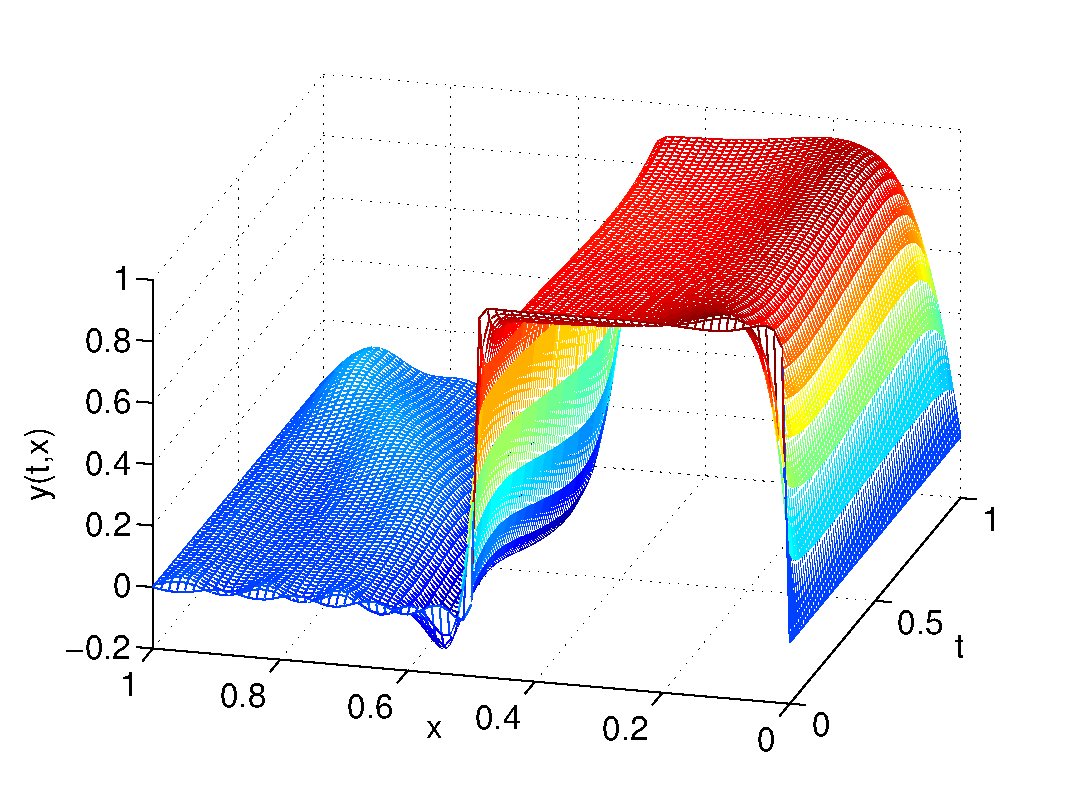
\includegraphics[width=0.49\textwidth]{plots/controlRedk5}}\hfill
%\subfloat[$k=10$]{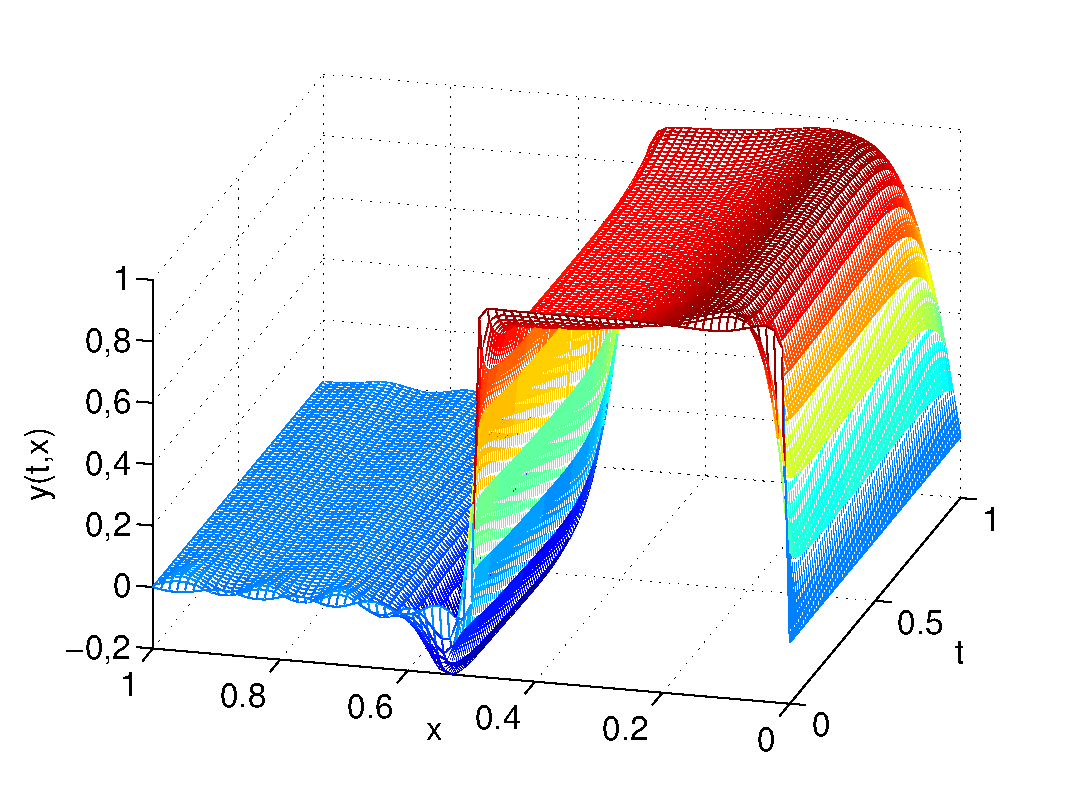
\includegraphics[width=0.49\textwidth]{plots/controlRedk10}}\\
%\caption{Reduced-order optimization.}\label{optRed}
%\end{figure}

%\begin{figure}[H]
%\centering
%\subfloat[$k=1$ (initial)]{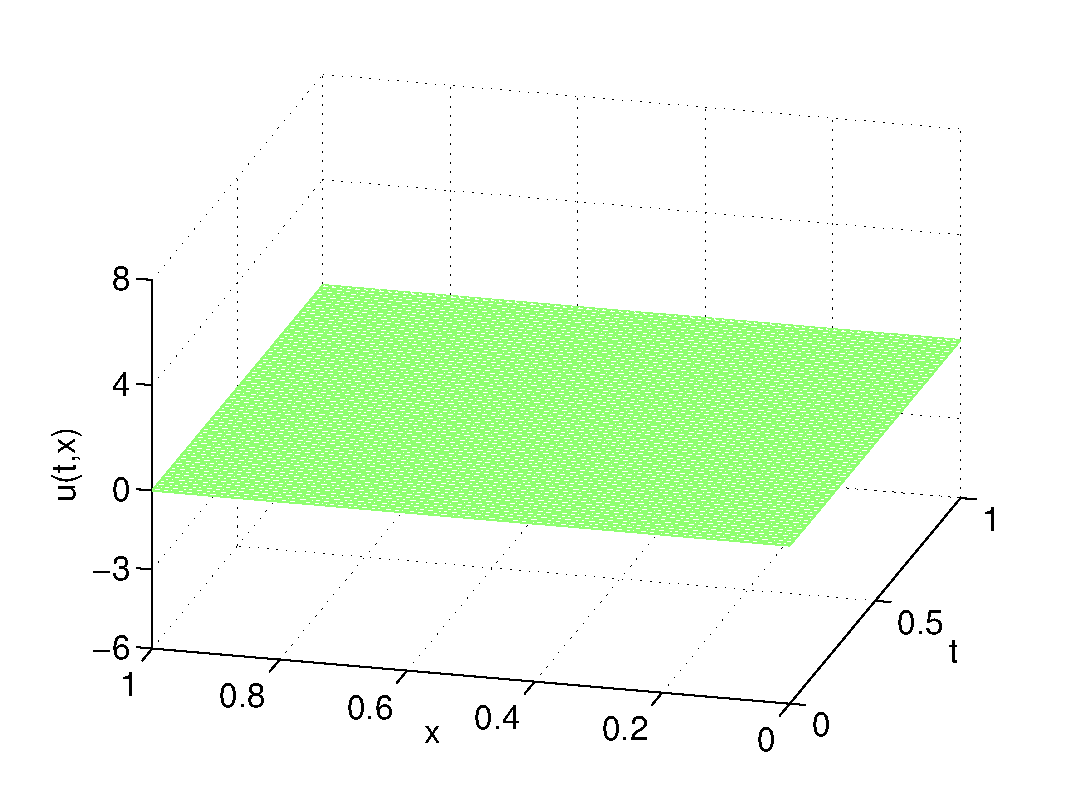
\includegraphics[width=0.49\textwidth]{plots/uRedk1}}\hfill
%\subfloat[$k=2$]{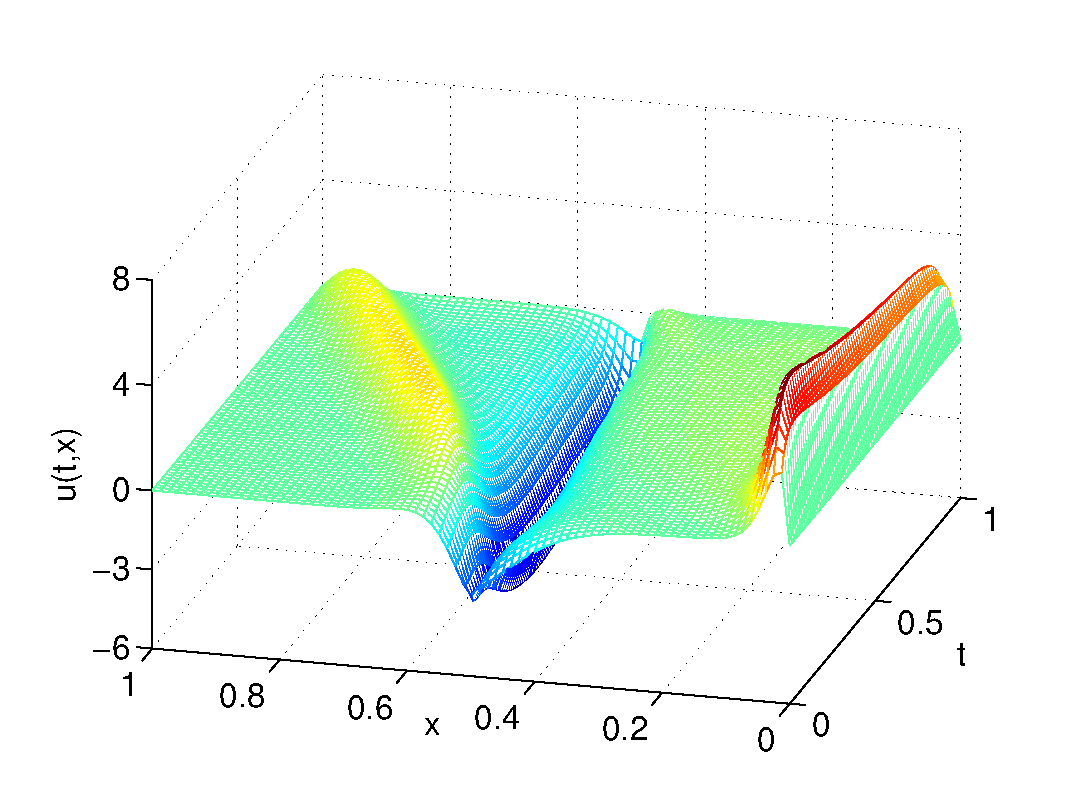
\includegraphics[width=0.49\textwidth]{plots/uRedk2}}\\
%\subfloat[$k=5$ ]{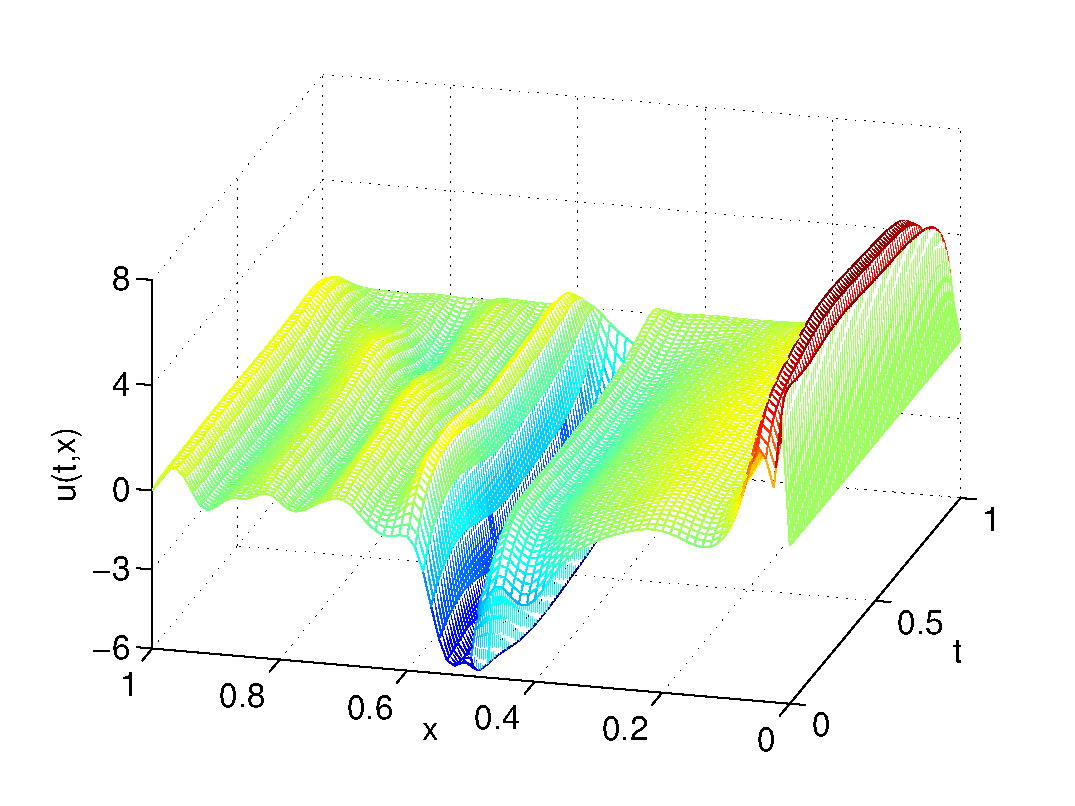
\includegraphics[width=0.49\textwidth]{plots/uRedk5}}\hfill
%\subfloat[$k=10$]{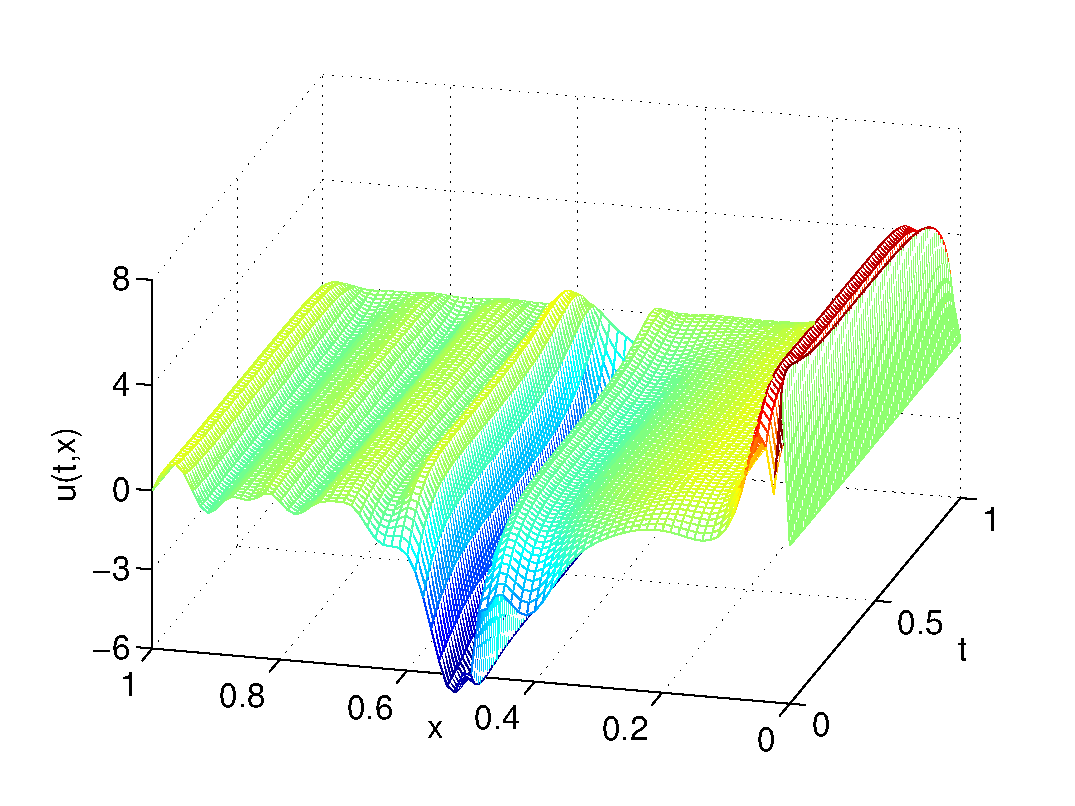
\includegraphics[width=0.49\textwidth]{plots/uRedk10}}\\
%\caption{Reduced-order control.}\label{optRedu}
%\end{figure}
\section{Low-dimensional control using individual control points}
\label{smallu_sec}
In order to overcome the dependence of the control on the dimension of the full-order model, we will restrict the control to certain discrete \textit{control points}. In Figure \ref{smallu}, we have indicated that we allow to control the system at only three different points in $[0,L]$. This approach requires, of course, some physical inside of the problem in the sense that we need to know at which points it is important to control the state.
\begin{figure}[H]
\centering
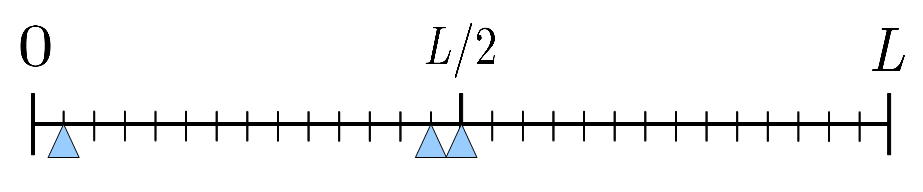
\includegraphics[width=0.49\textwidth]{plots/smallu.png}
\caption{Discretization of the interval $[0,L]$ indicating only $3$ discrete positions for control.}\label{smallu}
\end{figure}
We can model this approach by writing the control in the following way:
\begin{align}
\label{lowDimu}
\mathbf{u}(t) = \Psi_{n_c} \mathbf{\tilde u}(t), \quad \text{with } \mathbf{\tilde u}(t) \in \mathbb{R}^{n_c},
\end{align}
where $\mathbf{\tilde u}(t)$ is low-dimensional and contains only non-zero values of the control at the $n_c$ considered points. The matrix $\Psi$ indicates which entries of the control we want to consider. For the case in Figure \ref{smallu} with $n_c  = 3$, we would have:
\begin{align*}
\Psi_3 = \begin{pmatrix} 1 & 0 & 0 \\
                           &   \vdots & \\
                         0 & 1 & 0  \\
                         0 & 0 & 1  \\
                           &  \vdots &  \end{pmatrix} \in \mathbb{R}^{N \times 3}.
\end{align*}
Note that this decomposition corresponds to an ansatz:
\begin{align*}
u(t,x) \approx \sum_{j \in \mathcal{I}_{c}} u_j(t) \phi_j(x),
\end{align*}
with an index set $\mathcal{I}_{c}$ containing $n_c$ indices of the control points. This way, the mass matrix for the control can be derived in a straightforward way but the approach of \eqref{lowDimu} shows the gain in dimension reduction better: When we plug in \eqref{lowDimu} into the discretized objective function \eqref{redOpt}, we obtain:
\begin{align}
\label{redOpt_smallu}
\min_{\mathbf{\tilde{u}}_0,...,\mathbf{\tilde{u}}_{N_t}} \tilde{J}(\mathbf{\tilde y}_0,...,\mathbf{\tilde y}_{N_t},\mathbf{\tilde{u}}_0,...,\mathbf{\tilde{u}}_{N_t}) = \min_{\mathbf{\tilde{u}}_1,...,\mathbf{\tilde{u}}_{N_t}} \sum_{i=0}^{N_t} \delta \! t \left( \frac{1}{2} \mathbf{\tilde y}_i^T \mathbf{\tilde y}_i - \mathbf{\tilde z}^T\mathbf{\tilde y}_i + \frac{\omega}{2}\mathbf{\tilde{u}}_i^T \underbrace{\Psi^T M \Psi}_{\text{pre-compute}} \mathbf{\tilde{u}}_i \right),
\end{align}
which does not depend on the full-order dimension $N$ at all because the matrix $\Psi^T M \Psi \in \mathbb{R}^{n_c \times n_c}$. Note also that this matrix can be pre-computed. In the same way, we have for the discretized reduced Burgers' equation \eqref{redBurgers} the following:
\begin{align}
\label{redBurgers_smallu}
\tilde{c}_i(\mathbf{\tilde y}_i,\mathbf{\tilde y}_{i+1},\mathbf{\tilde u}_{i+1}) \equiv \frac{1}{\delta \! t} \mathbf{\tilde y}_{i+1} - \frac{1}{\delta \! t}\mathbf{\tilde y}_i + \frac{1}{2} \tilde{B}(\tilde{F}\mathbf{\tilde y}_{i+1})^2 + \nu \tilde{C}\mathbf{\tilde y}_{i+1} - \mathbf{\tilde f} - \underbrace{\Phi_\ell^T M \Psi}_{\text{pre-compute}} \mathbf{\tilde u}_{i+1} = 0,
\end{align}
where $i=0,...,N_t-1$ and $\Phi_\ell^T M \Psi \in \mathbb{R}^{\ell \times n_c}$.

In Figure \ref{result_Smallu}, we show the numerical result for $n_c = 3$. We see that even a control at only three different control points leads to a reasonable approximation to the desired state. We also present the corresponding control that drives the solution to the POD-DEIM reduced Burgers' equation into the desired state.
\begin{figure}[H]
\centering
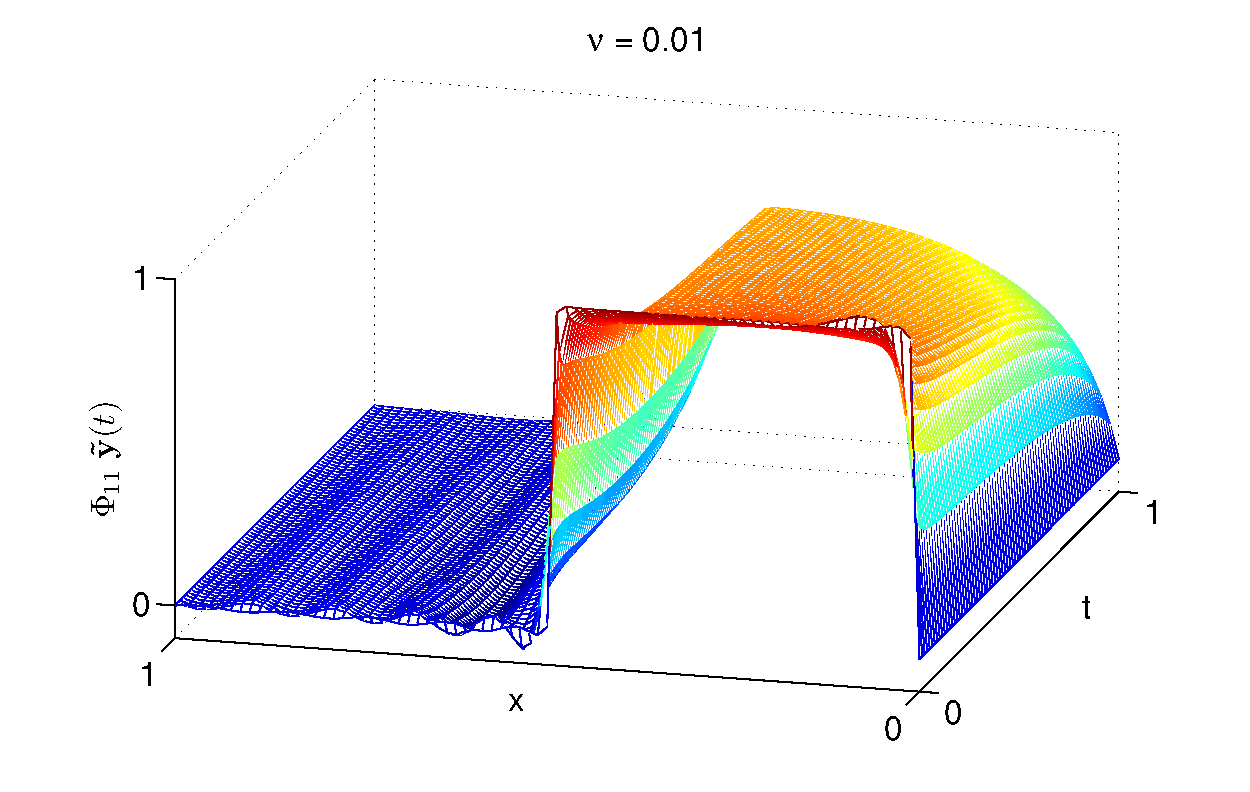
\includegraphics[width=0.49\textwidth]{plots/y_smallu} \hfill
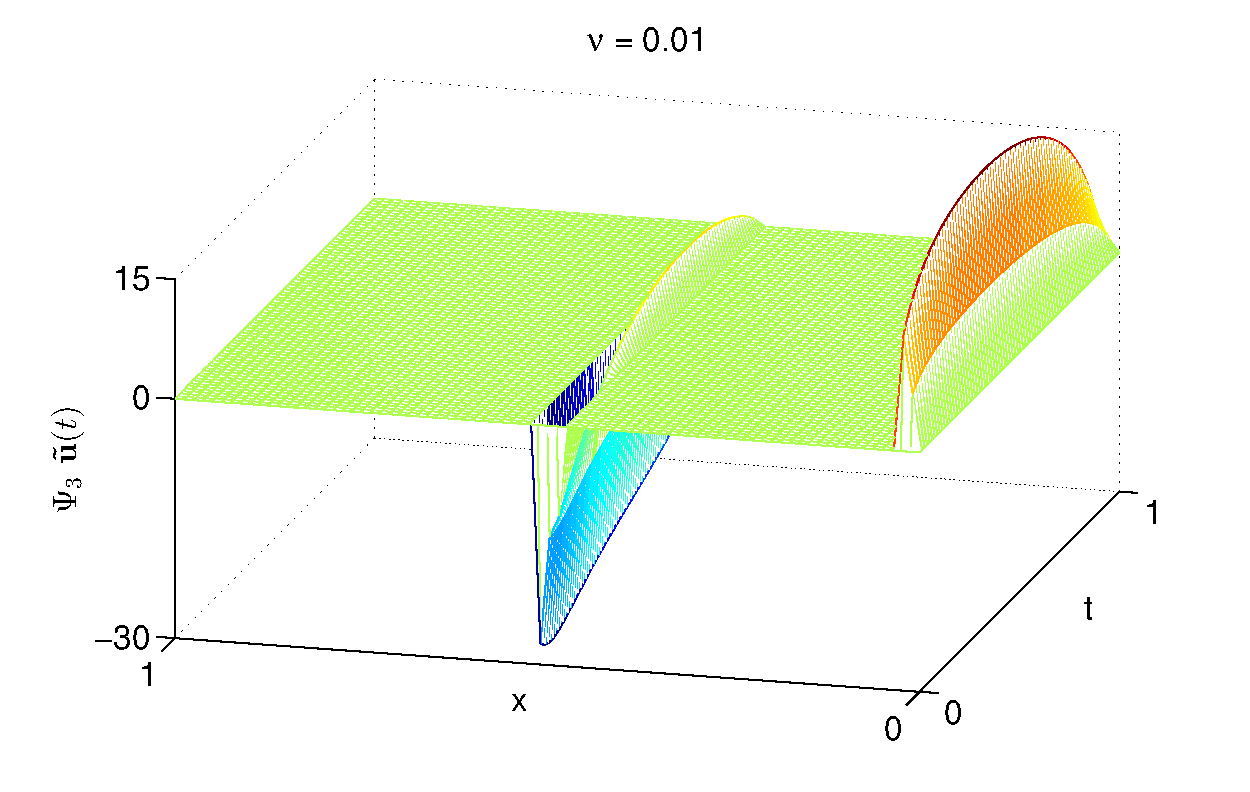
\includegraphics[width=0.49\textwidth]{plots/u_smallu}
\caption{Optimal control (right) and corresponding state (left) for $\ell = m = 11$ and $n_c = 3$ control points.}\label{result_Smallu}
\end{figure}
\section{Performance and error analysis}
\label{numTests}
The main goal of this thesis work is to evaluate the performance of POD-DEIM when applied to optimal control of Burgers' equation. In order to compare the results of the optimization using a POD-DEIM reduced model with the optimization based on a reduced model obtained from a pure POD reduction as suggested in \cite{KV99}, it is important to specify identical stopping criteria and tolerances for the respective numerical optimization algorithm. In this section, we present numerical results for three different viscosity parameters, $\nu = \{0.01, 0.001, 0.0001\}$, and for the three different optimization algorithms Newton-type, BFGS and SPG as presented in Section \ref{optAdj}, \ref{BFGS_section} and \ref{SPG_chap}, respectively. Since all three optimization algorithms are iterative methods, we are able to define a stopping of the optimization when either the change in the objective function is smaller than the tolerance $\varepsilon_\mathcal{J}$ or the zero-gradient condition is fulfilled upto a numeric tolerance specified by $\varepsilon_\nabla$. For the presented results of this section, we used  $\varepsilon_\mathcal{J} =$ \texttt{10e-8} and $\varepsilon_\nabla =$ \texttt{10e-9} in the respective Algorithms \ref{alg:Opt}, \ref{alg:BFGS} or \ref{alg:SPG}. In general, it is difficult to design a \textit{fair} comparison between different algorithms. For example, the stopping criterion for the gradient is implemented differently for the SPG method, see line $5$ of Algorithm \ref{alg:SPG}. Therefore, we also used a criterion which is called \textit{targeting} and which provides comparable results by choosing all parameters in such a way that the final value of the reduced objective function and the objective function of the full-order model are close. Moreover, we have required the error of the optimal state in the relative $L_2$-norm to be small.

In order to compare the optimal control of the POD and the POD-DEIM reduced Burgers' model, we are first interested in the \textit{accuracy} of the optimal state obtained by the two reduced models in comparison to the full-order optimal control as described in Section \ref{fullOrderControl}. Therefore, we choose the viscosity parameter $\nu = 0.01$ which requires a dimension of $N = 80$ for the full-order model, cf. Section \ref{fullOrderControl}. For a comparison of the optimal state obtained by a POD and POD-DEIM, we choose the DEIM-dimension constant, $m = 15$, and increase the POD dimension $\ell$ from $3$ to $25$. In Figure \ref{YerrL2}, we present the distribution of the error which is defined as the squared difference of the final state of the full-order optimization and the final state of the respective optimization of the reduced model,
\begin{align*}
 e(t,x) := [y(t,x) - \Phi_\ell \tilde{y}(t)]^2.
\end{align*}
Figure \ref{YerrL2} shows the error as a function of time and space for three different POD dimensions, $\ell = \{5,15,25\}$. We see that the error is large where the desired state is not smooth, i.e. at the boundary of the step function $z$. Furthermore, the plot in Figure \ref{YerrL2} shows that the error decreases as the POD dimension increases. For all three cases considered, the error is generally larger for the POD-DEIM reduced model but it is always of the same order of magnitude.
\begin{figure}[H]
\centering
\subfloat[$\ell = 5$]{\includegraphics[width=0.33\textwidth]{plots/YerrL2_pod_5_new}}\hfill
\subfloat[$\ell = 15$]{\includegraphics[width=0.33\textwidth]{plots/YerrL2_pod_15_new}}\hfill
\subfloat[$\ell = 25$]{\includegraphics[width=0.33\textwidth]{plots/YerrL2_pod_25_new}}\hfill \\
\subfloat[$\ell = 5$]{\includegraphics[width=0.33\textwidth]{plots/YerrL2_poddeim_5_new}}\hfill
\subfloat[$\ell = 15$]{\includegraphics[width=0.33\textwidth]{plots/YerrL2_poddeim_15_new}}\hfill
\subfloat[$\ell = 25$]{\includegraphics[width=0.33\textwidth]{plots/YerrL2_poddeim_25_new}}\hfill \\
\caption{Error distribution of the optimal state obtained by the Newton-type method and a POD and POD-DEIM reduced model.}\label{YerrL2}
\end{figure}
\newpage
In Figure \ref{L2err}, we present the error in the two reduced optimal sates with respect to the full optimal state not as a function of time and space but calculated in the corresponding $L_2$-norm. Since the POD reduced model only depends on $\ell$, we have again chosen a fixed DEIM-dimension $m = 15$ in order to compare the error in $L_2$ as a function of $\ell$. In Figure \ref{L2err}, we see that, as expected, the POD-DEIM error is larger for all considered $\ell$. It is also interesting to note that for $\ell > m$, the error of the POD-DEIM optimal state is dominated by the DEIM approximation error and does not decrease further whereas the error of the optimal state obtained from the POD reduced model still decreases.
\begin{figure}[H]
\centering
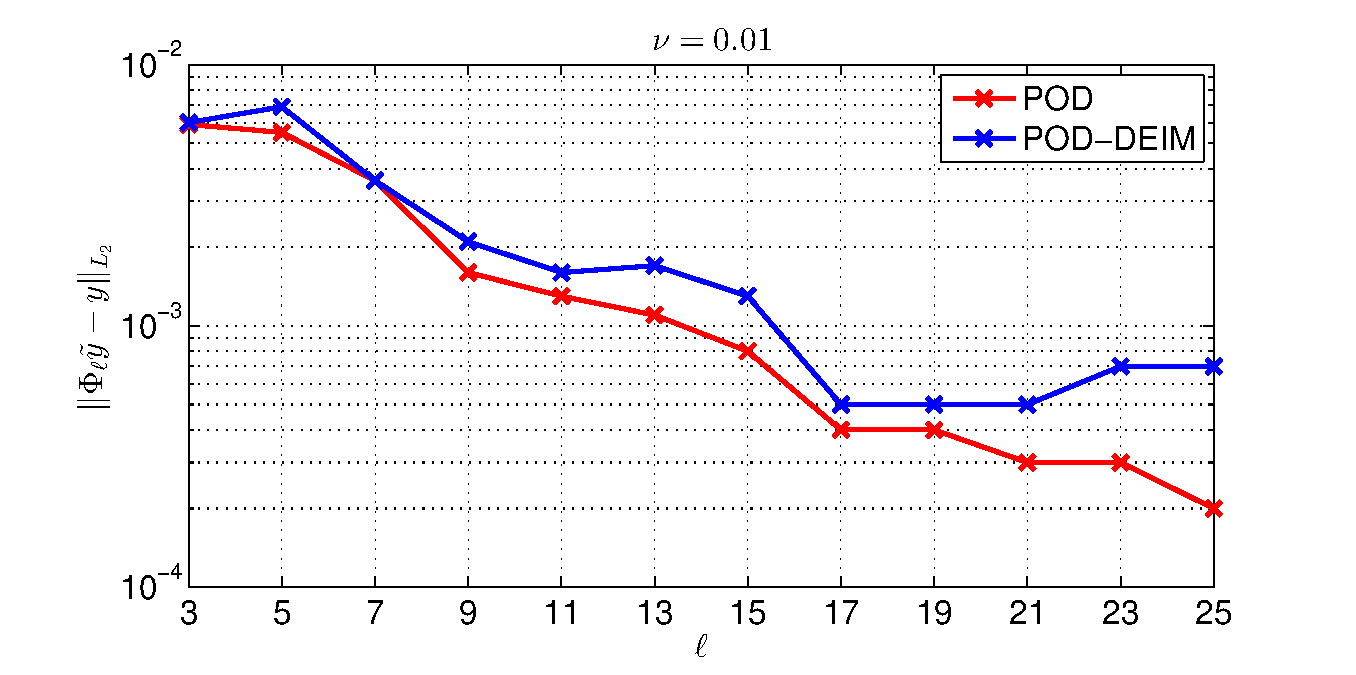
\includegraphics[width=0.66\textwidth]{plots/yL2err}
%\subfloat{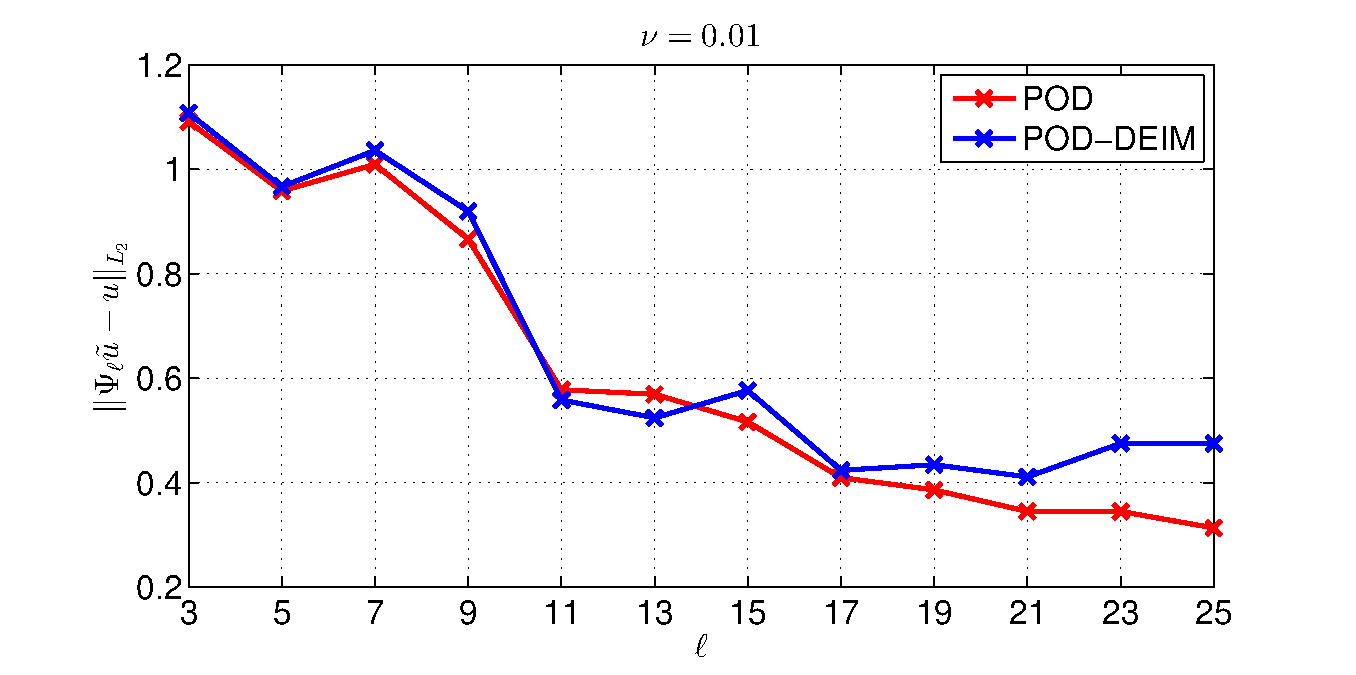
\includegraphics[width=0.7\textwidth]{plots/uL2err}}
\caption{Comparison of the $L_2$-error of the POD and the POD-DEIM approximation when the projection dimensions are increased.}\label{L2err}
\end{figure}
The results presented in Figure \ref{YerrL2} and Figure \ref{L2err} show that the POD-DEIM reduced optimal control problem \eqref{redOpt}-\eqref{redBurgers} yields to a comparable optimal solution to a POD-reduced model and the full-order optimal control problem \eqref{minJ_discr}-\eqref{Burgers2_discr}. We will next consider the application of the Newton-type optimization method of Algorithm \ref{alg:Opt} to the three different models with respect to computational time. Therefore, we have calculated the optimal solution for three different values of $\nu$ in Table \ref{time_messure1}. The measurements reported in Table \ref{time_messure1} are:
\begin{itemize}
 \item $N$/$\ell$/$m$ - The (spatial) dimension of the full-order, POD and POD-DEIM reduced model, respectively. In the case of POD-DEIM we present both reduced dimensions as the tuple $(\ell,m)$
 \item $t_{opt}[s]$ - This is the time needed for the considered optimization algorithm. In case of the reduced optimal control presented in Algorithm \ref{alg:Opt+MOR1}, this also includes the time which is necessary for building the reduced model, i.e. the pre-computation of the POD basis and DEIM-indices.
 \item $\mathcal{J}(y^*,u^*)$ - The value of the (reduced) objective function after convergence of the optimization iteration.
 \item $\bar{e}$ - The relative error as defined in \eqref{relErr_def}, computed for the optimal state.
 \item $S_P$ - The speedup in computation time.
\end{itemize}
\newpage
\begin{table}[H]
\centering
\begin{tabular}{|c|c|c|c|c|c|c|c|c|c|}
\cline{1-10}
 & \multicolumn{3}{ c| }{$\nu = 0.01$} & \multicolumn{3}{ c| }{$\nu = 0.001$}& \multicolumn{3}{ c| }{$\nu = 0.0001$}\\ \cline{2-10}
 & Full & POD & DEIM & Full & POD & DEIM & Full & POD & DEIM \\ \cline{1-10}
$N$/$\ell$/$m$ & $80$ &$ 9 $&$(9,25)$ &$200$ &$11$ &$(11,25)$ & $800$&$15$ & $(15,25)$\\ \cline{1-10}
$t_{opt}[s]$        & 4.83      &4.13      &3.22       & 23.1 & 6.38 & 5.25 & 1,865.8 & 23.61 & 18.42 \\ \cline{1-10}
$\mathcal{J}(y^*,u^*)$   &  0.0241      & 0.0262      &0.0233        & 0.0206 & 0.0198 & 0.0200 &0.0202 & 0.0191 &0.0233 \\ \cline{1-10}
$\bar{e}$ &- & 0.0097 &  0.0141&- & 0.0194 & 0.0192 &- & 0.0255 &  0.0238\\ \cline{1-10}
$S_P$           & -      &1.35       &1.9  & - &  3.7 & 4.4 & - & \textbf{79.0} &\textbf{101.3}\\ \cline{1-10}
\end{tabular}
\caption{Results of the Newton-type optimization method \ref{alg:Opt} for $\nu = \{0.01, 0.001, 0.0001\}$.}\label{time_messure1}
\end{table}
The results in Table \ref{time_messure1} show that for all values of $\nu$, the POD as well as the POD-DEIM reduced optimal control problem lead to an optimal solution such that the value of the objective function $\mathcal{J}(y^*,u^*)$ is similar. We further note that the optimal state of the reduced model is a good approximation for the optimal state of the full-order optimization problem which can be seen by a small relative error, $\bar{e} \in \mathcal{O}(10^{-2})$, for all considered settings. The most important conclusion from Table \ref{time_messure1} is that for all three values of $\nu$, the speedup of the POD-DEIM reduced model is larger than the speedup of the POD-reduced model. In the case of $\nu = 0.0001$, the large full-order dimension $N$ that is required for numerical stability even leads to a computational speedup of $\sim 80$ for the POD-reduced optimization compared to a speedup of more than $100$ for the POD-DEIM reduced optimal control problem.

In the next numerical test we consider the same setting as before but we use the approach of a low-dimensional control as described in Section \ref{smallu_sec}. For the results presented in Table \ref{time_messure2}, we used $n_c = 3$ control points at the positions as indicated in Figure \ref{smallu}. Since for the time discretization of the interval $[0,1]$ we needed to choose $N_t = 80$ equidistant time-steps, the choice of $n_c =3$ has the consequence that the optimization in \eqref{redOpt_smallu} can be formulated in the unknown $\underline{\mathbf{\tilde u}} := [\mathbf{\tilde u}_1,...,\mathbf{\tilde u}_{N_t}]^T$ which is a vector of dimension $240$. In Table \ref{time_messure2}, we first note that the value of the objective function is higher for all models and all values of $\nu$ compared to Table \ref{time_messure1}. This is expected since we only allow the control to be different from zero at three discrete positions and, therefore, it is not possible to drive the solution of Burgers' equation into the desired state with the same accuracy as before. At the same time, we see that the computational cost for all presented simulations is much less than in Table \ref{time_messure1} due to the lower dimension of the respective optimization problem. Again, the approximation of the optimal state obtained when using the reduced order optimization is of good quality as the small relative error indicates, $\bar{e} \in \mathcal{O}(10^{-2})$. The speedup obtained by the dimension reduction of POD and POD-DEIM is generally smaller in this case compared to the previous experiment but, again, we can see an improvement obtained by the application of DEIM.
\begin{table}[H]
\centering
\begin{tabular}{|c|c|c|c|c|c|c|c|c|c|}
\cline{1-10}
 & \multicolumn{3}{ c| }{$\nu = 0.01$} & \multicolumn{3}{ c| }{$\nu = 0.001$}& \multicolumn{3}{ c| }{$\nu = 0.0001$}\\ \cline{2-10}
 & Full & POD & DEIM & Full & POD & DEIM & Full & POD & DEIM \\ \cline{1-10}
$N$/$\ell$/$m$ & $80$&$9$ &$(9,25)$ &$200$ &$11$ &$(11,25)$ &$800$ & $15$ & $(15,25)$\\ \cline{1-10}
$t_{opt}[s]$   &3.68 &2.41 & 1.90& 5.44 &2.6 & 1.89& 117.32 & 8.17 & 6.10 \\ \cline{1-10}
$\mathcal{J}(y^*,u^*)$ &0.0300 & 0.0394&  0.0396&0.0348 &0.0439 & 0.0371 &0.0763 & 0.0865& 0.0893\\ \cline{1-10}
$\bar{e}$   & -&0.0132 &  0.0142& -& 0.0127&  0.0187&- & 0.0204& 0.0304\\ \cline{1-10}
$S_P$           & - &1.6 & 1.9 & - & 2.0 & 2.9& - &  14.4 &  19.2\\ \cline{1-10}
\end{tabular}
\caption{Results of the Newton-type optimization method \ref{alg:Opt} using a low-dimensional control with $n_c = 3$ and $\nu = \{0.01, 0.001, 0.0001\}$.}\label{time_messure2}
\end{table}
As a last numerical test, we want to compare the second-order Newton-type method \ref{alg:Opt} to the first-order methods BFGS and SPG, as presented in Section \ref{BFGS_section} and \ref{SPG_chap}, respectively. In our experiments, the same stopping criteria have been used for all three iterative methods. In Table \ref{time_messure3}, we present the results of the three optimization algorithms for the optimal control of Burgers' equation and the respective results for the POD/DEIM reduced models when the viscosity parameter is $\nu = 0.0001$ and a control is only possible at $n_c = 3$ control points. We have chosen the smallest $\nu$ because for this case we have previously seen the largest speedup. Table \ref{time_messure3} shows almost the same speedup for all three optimization algorithms when compared to the full-order solution. Note that the results in Table \ref{time_messure3} show that the value of the objective function was slightly lower for the full-order model in all three cases which indicates that the reduced models do not reach entirely the optimal state of the full model.
\begin{table}[H]
\centering
\begin{tabular}{|c|c|c|c|c|c|c|c|c|c|}
\cline{1-10}
 & \multicolumn{3}{ c| }{Newton-type} & \multicolumn{3}{ c| }{BFGS}& \multicolumn{3}{ c| }{SPG}\\ \cline{2-10}
 & Full & POD & DEIM & Full & POD & DEIM & Full & POD & DEIM \\ \cline{1-10}
$N$/$\ell$/$m$ &$800$ & $15$ & $(15,25)$ & $800$ & $15$ & $(15,25)$ & $800$ & $15$ & $(15,25)$ \\ \cline{1-10}
$t_{opt}[s]$   &117.32 & 8.17 & 6.10& 294.90& 15.64 & 14.38& 123.00&  7.61 & 16.11\\ \cline{1-10}
$\mathcal{J}(y^*,u^*)$ &0.0763 & 0.0865& 0.0893&0.0840 &  0.0879 &0.0857 &0.0763 & 0.0861 & 0.0878\\ \cline{1-10}
$\bar{e}$   &- & 0.0204& 0.0304 &- &  0.0226&0.0247 &- & 0.0218& 0.0355\\ \cline{1-10}
$S_P$           & - & 14.4 &  19.2& - & 18.3& 20.5& - & 16.3& 7.6\\ \cline{1-10}
\end{tabular}
\caption{Results of three different optimization algorithms and $\nu = 0.0001, n_c = 3$.}\label{time_messure3}
\end{table}
We note in Table \ref{time_messure3} that the speedup for the POD-DEIM reduced model is small when the SPG method is applied. This can be explained when taken into account the number of evaluations of the cost function \eqref{redOpt} and its gradient in Table \ref{time_messure3_eval}. We see that in order to converge within the same precision, the SPG method needs $52$ evaluations of the objective function when POD-DEIM has been applied. This analysis explains the relatively poor speedup of $7.6$ for POD-DEIM compared to a speedup of $16.3$ of POD. The much larger number of required function evaluations overtops the speedup of a single iteration.
\begin{table}[H]
\centering
\begin{tabular}{|c|c|c|c|c|c|c|}
\cline{1-7}
 & \multicolumn{3}{ c| }{BFGS}& \multicolumn{3}{ c| }{SPG}\\ \cline{2-7}
 & Full & POD & DEIM & Full & POD & DEIM \\ \cline{1-7}
$\# \mathcal J$ &65 &38 & 40&17 & 13& 52 \\ \cline{1-7}
$\# \nabla \mathcal J$ &65 & 38&40 &16 &12 &12 \\ \cline{1-7}
\end{tabular}
\caption{Number of evaluations of the cost function and the gradient for the first-order methods in the setting of Table \ref{time_messure3}.}\label{time_messure3_eval}
\end{table}
Moreover, the SPG method has been considered for three different values of $\nu$ and the full-dimensional control that has been constrained in the following way, $-2 \leq u \leq 2$. In Section \ref{SPG_chap}, we have defined a projector that allows to include this bound constraint in an easy way. The numerical results presented in Table \ref{time_messure4} show a larger value of the objective function at the optimal state compared to the results obtained by the Newton-type method presented in Table \ref{time_messure1}. This shows that the restriction of the control to be within a certain range influences the quality of the obtained optimal state. Again, the performed numerical tests show that the reduced models approximate the optimal state of the full-order model well since $\bar{e} \in \mathcal{O}(10^{-2})$. For the smallest value of $\nu = 0.0001$ which corresponds to a full-order dimension of $N=800$, we observe a speedup of the SPG method of $3.6$ when POD is used to solve the constraining Burgers' equation and a speedup of $8.8$ in the case of a model order reduction by POD-DEIM while the value of the objective function for both reduced models has been almost the same.
\begin{table}[H]
\centering
\begin{tabular}{|c|c|c|c|c|c|c|c|c|c|}
\cline{1-10}
 & \multicolumn{3}{ c| }{$\nu = 0.01$} & \multicolumn{3}{ c| }{$\nu = 0.001$}& \multicolumn{3}{ c| }{$\nu = 0.0001$}\\ \cline{2-10}
 & Full & POD & DEIM & Full & POD & DEIM & Full & POD & DEIM \\ \cline{1-10}
$N$/$\ell$/$m$ & $80$ &$ 9 $&$(9,25)$ &$200$ &$11$ &$(11,25)$ & $800$&$15$ & $(15,25)$\\ \cline{1-10}
$t_{opt}[s]$   &6.61 & 4.02 & 3.77&  12.55&  6.61 & 5.99& 193.40& 53.16 & 22.05\\ \cline{1-10}
$\mathcal{J}(y^*,u^*)$ & 0.0367 & 0.0399&  0.0332&0.0347 & 0.0397 & 0.0378& 0.0339 & 0.0357 &  0.0367\\ \cline{1-10}
$\bar{e}$   &- & 0.0193& 0.0250&- & 0.0255& 0.0249&- & 0.0238&  0.0248\\ \cline{1-10}
$S_P$           & - &1.6 &  1.8& - &1.9 &2.1 & - & 3.6& 8.8\\ \cline{1-10}
\end{tabular}
\caption{Results of the SPG method and a bounded control $-2 \leq u \leq 2$.}\label{time_messure4}
\end{table} 